\chapter{Business architecture}
\label{sec:business-architecture}
	
	% rewrite
	This chapter addresses the business architecture aiming to describe the internal processes, events and roles answering questions concerning who shall do what and when.
	
	This chapter first presents the baseline business architecture, as it is currently established and, then, presents a new (target) business architecture, as it is envisaged in the light of the digital transformation moving towards goals identified in the motivation structure (Section \ref{sec:motivation-architecture}). The new business processes (see Section \ref{sec:lifecycle-new}) are aligned with use case descriptions from Section \ref{sec:business-use cases}. The latter are derived from materials describing the current workflow and interviews with the SU technical and business team members.

	Beforehand, however, the description commences by explaining how a prototypical business architecture is structured that will serve as framework to better understand the diagrams in this chapter. 	
	
	\section{Prototypical business structure}
	
	Following the metaphor of layers presented in the motivation view (see Section \ref{sec:how-to-motivation}), the organisation of business structure is also explained in terms of layers. Figure \ref{fig:business-structure-protopypical} depicts three layers with the most important elements of the business structure. 
	
	\begin{figure}[h]
		\centering
		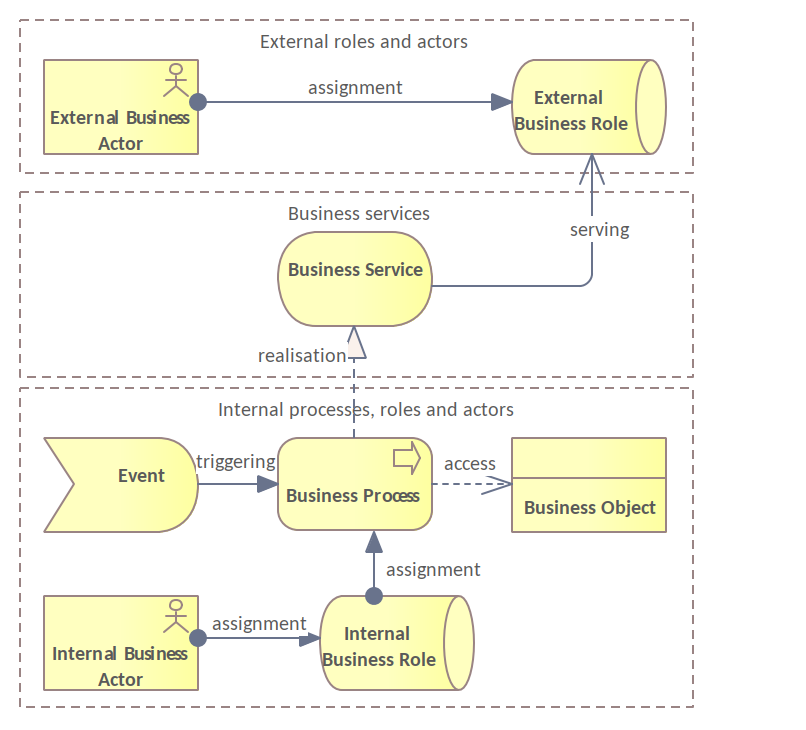
\includegraphics[width=0.7\textwidth]{images/views/Business view.png}
		\caption{The prototypical business structure view}
		\label{fig:business-structure-protopypical}
	\end{figure} 
	
	The topmost layer accounts for the external players or \textit{actors}, which represent a business entity that is capable of performing behaviour and \textit{roles}, which represent skills and responsibilities for performing specific behaviour, and to which an actor can be assigned \citep{archimate3.1}. 
	
	The middle layer represents the \textit{services} that are offered by the organisation to external players. A business service represents explicitly-defined behaviour that a business role, business actor or business collaboration exposes to its environment \citep{archimate3.1}.
	
	The lower layers accounts for the internal organisation in terms of \textit{events}, \textit{roles}, \textit{processes} and \textit{objects}. The business process represents a sequence of business behaviours that achieves a specific result such as a defined set of products or business services. The business event represents an organisational state change; while a business object represents a (passive) concept used within a particular business domain.
	
	\section{Organisation structure}
	
	